\documentclass[12pt,a4paper]{report}

\usepackage[utf8]{inputenc} % pentru suport diacritice
\renewcommand\familydefault{\sfdefault} % sans serif

\usepackage[margin=2.54cm]{geometry} % dimensiuni pagină și margini
\usepackage{graphicx} % support the \includegraphics command and options

% formatting sections and subsections
\usepackage{textcase}
\usepackage[titletoc, title]{appendix}
\usepackage{titlesec}
\titleformat{\chapter}{\large\bfseries\MakeUppercase}{\thechapter}{2ex}{}[\vspace*{-1.5cm}]
\titleformat*{\section}{\large\bfseries}
\titleformat*{\subsection}{\large\bfseries}
\titleformat*{\subsubsection}{\large\bfseries}

\usepackage{chngcntr}
\counterwithout{figure}{chapter} % no chapter number in figure labels
\counterwithout{table}{chapter} % no chapter number in table labels
\counterwithout{equation}{chapter} % no chapter number in equation labels

\usepackage{booktabs} % for much better looking tables
\usepackage{url} % Useful for inserting web links nicely
\usepackage[bookmarks,unicode,hidelinks]{hyperref}

\usepackage{array} % for better arrays (eg matrices) in maths
\usepackage{paralist} % very flexible & customisable lists (eg. enumerate/itemize, etc.)
\usepackage{verbatim} % adds environment for commenting out blocks of text & for better verbatim
\usepackage{subfig} % make it possible to include more than one captioned figure/table in a single float
\usepackage{enumitem}
\setlist{noitemsep}

% packages used for citations
\usepackage{apacite}
\usepackage{natbib}

\usepackage{xcolor}
\usepackage{listings}
\lstset{language=Python,basicstyle={\bfseries \color{black}},keywordstyle={\bfseries \color{blue}}}

%%% HEADERS & FOOTERS
\usepackage{fancyhdr}
\pagestyle{empty}
\renewcommand{\headrulewidth}{0pt}
\renewcommand{\footrulewidth}{0pt}
\lhead{}\chead{}\rhead{}
\lfoot{}\cfoot{\thepage}\rfoot{}

\newcommand{\HeaderLineSpace}{-0.25cm}

\newcommand{\UniTextEN}{National University of Science and Technology POLITEHNICA Bucharest\\
Faculty of Automatic Control and Computers\\
Computer Science and Engineering Department\\}
\newcommand{\DiplomaEN}{DIPLOMA PROJECT}
\newcommand{\AdvisorEN}{Thesis advisors:}
\newcommand{\BucEN}{BUCHAREST}

\newcommand{\frontPage}[7]{
\begin{titlepage}
\begin{center}
{\Large #1}  % header (university, faculty, department)
\vspace{50pt}
% TODO: add pics/ logos if available
% \begin{tabular}{ccc}
% \includegraphics[height=3cm]{pics/UNST Poli.png} & 
% \includegraphics[height=3cm]{pics/A&C.png} & 
% \includegraphics[height=3cm]{pics/UPB NLP.png}
% \end{tabular}

\vspace{105pt}
{\Huge #2}\\                             % diploma project text
\vspace{40pt}
{\Large #3}\\ \vspace{0pt}               % project title
\vspace{20pt}
{\large #4}\\                            % project subtitle
\vspace{40pt}
{\LARGE \Name}\\                         % student name
\end{center}
\vspace{60pt}
\begin{tabular*}{\textwidth}{@{\extracolsep{\fill}}p{6cm}r}
&{\large\textbf{#6}}\vspace{10pt}\\      % scientific advisor
&{\large \AdvisorA}\\                    % advisor name A
&{\large \AdvisorB}                      % advisor name B
\end{tabular*}
\vspace{20pt}
\begin{center}
{\large\textbf{#7}}\\
\vspace{0pt}
{\normalsize \Year}
\end{center}
\end{titlepage}
}

\newcommand{\frontPageEN}{\frontPage{\UniTextEN}{\DiplomaEN}{\ProjectTitleEN}{\ProjectSubtitleEN}{\ProjectSubtitleEN}{\AdvisorEN}{\BucEN}}

\linespread{1.15}
\setlength\parindent{0pt}
\setlength\parskip{.28cm}

%% Abstract macro
\newcommand{\AbstractPage}{
\begin{titlepage}

\thispagestyle{fancy}\setcounter{page}{5}
\clearpage\phantomsection\addcontentsline{toc}{chapter}{Abstract}

\textbf{\large ABSTRACT}\par
\AbstractEN \vfill
\textbf{\large REZUMAT}\par
\AbstractRO\par\vfill
\end{titlepage}
}

%%%%%%%%%%%%%%%%%%%%%%%%%%%%%%%%%%%%%%%%%%%%%%%%%%
%%          End of template definitions
%%%%%%%%%%%%%%%%%%%%%%%%%%%%%%%%%%%%%%%%%%%%%%%%%%

\newcommand{\ProjectTitleEN}{Meme Captioning on memes900k: An Ablation of Visual Encoders and Caption Decoders}
\newcommand{\ProjectSubtitleEN}{A controlled comparison against DeepHumor}
\newcommand{\Name}{Mohammed Arsh}
\newcommand{\AdvisorA}{Prof. dr. ing. X}
\newcommand{\AdvisorB}{Prof. dr. ing. Y}
\newcommand{\Year}{2026}

\title{Diploma Project}
\author{\Name}
\date{\Year}

%%
%%   Câmpurile aferente rezumatului
%%
\newcommand{\AbstractEN}{
We train an image-to-text model to caption meme templates on the \textit{memes900k} dataset (900,000 captions across 300 templates), following \citet{deephumor2020}. We perform a controlled 2$\times$2 ablation over two frozen visual encoders (ResNet-50 \citep{he2016deep}, CLIP ViT-B/32 \citep{radford2021learning}) and two decoders (LSTM \citep{hochreiter1997lstm}, Transformer \citep{vaswani2017attention}), using a shared greedy decoder and reporting BLEU \citep{papineni2002bleu,post2018call} alongside perplexity on the official test split. At 1 epoch, the decoder dominates (LSTM$\to$Transformer gives +5.65 BLEU with CLIP), and encoder choice only matters when the decoder is weak. Behind a Transformer decoder, encoder and embedding size wash out (14.38--14.66 BLEU across all four 3-epoch runs). Three epochs roughly halve perplexity while BLEU stays flat, exposing the gap between teacher-forced fit and free-running generation. The contribution is a clean, reproducible measurement methodology rather than a new state of the art.
}

\newcommand{\AbstractRO}{Translation to be made at the end

\vspace{3\baselineskip}
\textbf{Keywords}: Image Captioning, Memes, Vision-Language Models, BLEU, Perplexity, DeepHumor
}

\begin{document}
\pagenumbering{roman}
\frontPageEN
\begingroup
\linespread{1}
\tableofcontents
\endgroup

\pagestyle{fancy}
\listoffigures\addcontentsline{toc}{chapter}{List of figures}
\begingroup
\let\clearpage\relax
\listoftables\addcontentsline{toc}{chapter}{List of tables}
\endgroup

\AbstractPage

\pagenumbering{arabic}

\chapter{Introduction}\pagestyle{fancy}
\label{ch:intro}

\section{Context}
\citet{deephumor2020} introduced \textit{DeepHumor}, an image-to-text approach for generating meme captions on \textit{memes900k} (300 templates, 900,000 captions). The public codebase reports teacher-forced perplexity and does not evaluate generated captions on a held-out test set with a reproducible decoder.

\section{Problem Statement}
We need a rigorous, controlled comparison: isolate visual encoder (ResNet-50 \citep{he2016deep} vs. CLIP \citep{radford2021learning}) and decoder (LSTM \citep{hochreiter1997lstm} vs. Transformer \citep{vaswani2017attention}) effects while using the same decoding and metrics, and evaluate on the official caption-level test split.

\section{Objectives}
\begin{itemize}
\item Run a 2$\times$2 ablation (ResNet-50/CLIP $\times$ LSTM/Transformer) with frozen encoders.
\item Report BLEU \citep{papineni2002bleu} on generated captions (shared greedy decoding) and perplexity, on the official test split.
\item Match a short budget (1 epoch = 6,250 steps) and a longer budget (3 epochs = 18,750 steps).
\item Produce a rendered caption gallery and a one-command inference demo.
\item Write a reproducible final report and deliverables.
\end{itemize}

\section{Thesis Structure}
Chapter~\ref{ch:sota} surveys image captioning and the DeepHumor reference. Chapter~\ref{ch:method} details data, encoders/decoders, and metrics. Chapter~\ref{ch:results} presents tiered results and qualitative outputs. Chapter~\ref{ch:discussion} discusses findings and limitations. Chapter~\ref{ch:conclusions} concludes and proposes future work. Appendix~\ref{app:repro} covers reproducibility.

\chapter{State of the art}
\label{ch:sota}

\section{Image captioning}
Early neural captioning models used CNN features with RNN decoders (\textit{Show and Tell}, \citealp{vinyals2015show}). Attention over spatial features improved grounding (\textit{Show, Attend and Tell}, \citealp{xu2015show}). The Transformer \citep{vaswani2017attention} replaced recurrence with self- and cross-attention, becoming a standard decoder in vision-language systems. Large-scale vision-language pretraining (e.g. CLIP, \citealp{radford2021learning}) provides semantically rich image representations that transfer well to captioning.

\section{Meme captioning and DeepHumor}
\citet{deephumor2020} trained frozen ResNet-50 + LSTM (and a Transformer variant) on \textit{memes900k}, using teacher-forced perplexity as the primary metric and an unseeded sampling-based decoder. We adopt the dataset and the frozen-feature paradigm but require test-set BLEU with a shared greedy decoder and explicit ablations.

\section{Metrics}
BLEU \citep{papineni2002bleu} measures n-gram overlap between generated and reference captions; \citet{post2018call} recommend clear reporting (here via sacrebleu). Perplexity under teacher forcing is informative within a tokenizer family but not directly comparable across vocabularies.

\chapter{Method}
\label{ch:method}

\section{Corpus}
\subsection{Descriptives}
\textit{memes900k} provides 300 meme template images and 900,000 tab-separated caption rows. We use the official caption-level split: 750,000 train, 75,000 val, 75,000 test. Every template appears in all splits; thus scores reflect \emph{new captions for seen templates}, not unseen templates.

\begin{table}[h]
\centering
\begin{tabular}{lrr}
\toprule
Split & Rows & Per template \\
\midrule
Train & 750,000 & 2,500 \\
Validation & 75,000 & 250 \\
Test & 75,000 & 250 \\
\bottomrule
\end{tabular}
\caption{Official caption-level split of \textit{memes900k}.}
\end{table}

\section{(Neural) Architecture}
\textbf{Encoders (frozen):} ResNet-50 \citep{he2016deep} yields a 49$\times$2048 spatial sequence; CLIP ViT-B/32 \citep{radford2021learning} yields a 50$\times$768 patch-token sequence. Features are precomputed once per template.

\textbf{Decoders:} LSTM \citep{hochreiter1997lstm} (hidden 512, 2 layers, embedding 256) with mean-pooled image features as initial state. Transformer \citep{vaswani2017attention} (6 layers, 8 heads, hidden 512, FFN 2048, embedding 512) with visual features as encoder memory and tied input/output embeddings.

The 2$\times$2: (ResNet-50/CLIP) $\times$ (LSTM/Transformer). Hyperparameter screening ranked CLIP+Transformer configs at 6,000 steps by validation loss; the embed-768 variant was confirmed at full budget.

\section{Performance Metrics}
\textbf{Perplexity:} $ppl=\exp(\textrm{mean NLL})$ under teacher forcing, computed over all 75,000 test rows. Only comparable within this project's GPT-2 BPE vocabulary.

\textbf{BLEU:} sacrebleu corpus BLEU on a fixed, seeded 5,000-row test sample with greedy decoding \citep{papineni2002bleu,post2018call}. This is the cross-tokenizer/comparative number.

\textbf{Budgets:} Tier 1 = 1 epoch = 6,250 steps (subsample 200k, batch 32, grad-accum 4, lr 3e-4, seed 42). Tier 2 = 3 epochs = 18,750 steps.

\chapter{Results}
\label{ch:results}

\section{Tier 1 -- 1 epoch (6,250 steps)}
\begin{table}[h]
\centering
\begin{tabular}{lcccc}
\toprule
Run & Encoder & Decoder & Test BLEU & Test perplexity \\
\midrule
A & ResNet-50 & LSTM & 2.13 & 255.5 \\
B & CLIP & LSTM & 8.92 & 259.7 \\
C & CLIP & Transformer & \textbf{14.57} & 71.5 \\
D & ResNet-50 & Transformer & 14.50 & 72.7 \\
E (confirmation) & CLIP & Transformer (embed 768) & 14.36 & \textbf{68.4} \\
\bottomrule
\end{tabular}
\caption{Tier 1 results (official test split).}
\end{table}

Decoder dominates: LSTM$\to$Transformer gives +5.65 BLEU (B$\to$C) and +12.37 (A$\to$D). Encoder matters only when decoder is weak (+6.79 A$\to$B) and is flat for the Transformer (C$\to$D = -0.07). Larger embedding (E) improves perplexity but not BLEU.

\section{Tier 2 -- 3 epochs (18,750 steps)}
\begin{table}[h]
\centering
\begin{tabular}{lcccc}
\toprule
Run & Encoder & Decoder & Test BLEU & Test perplexity \\
\midrule
A$'$ & ResNet-50 & LSTM & 13.36 & 115.9 \\
B$'$ & CLIP & LSTM & 12.16 & 120.7 \\
C$'$ & CLIP & Transformer & 14.38 & 54.7 \\
D$'$ & ResNet-50 & Transformer & 14.63 & 55.5 \\
E$'$ & CLIP & Transformer (embed 768) & \textbf{14.66} & 55.2 \\
\bottomrule
\end{tabular}
\caption{Tier 2 results (3 epochs).}
\end{table}

Transformer cluster is tight (14.38--14.66). LSTMs reach 12--13 but still trail. Perplexity roughly halves while BLEU is flat.

\section{Perplexity $\neq$ BLEU}
More training sharpens teacher-forced distributions but does not improve free-run captions --- the exposure-bias gap. Validation-loss ranking does not match BLEU ranking.

\section{Qualitative results}
Contact sheets (distinct templates) are shown in Figures~\ref{fig:emb}--\ref{fig:lstm}. Each card shows the template rendered with the generated caption and the gold caption for the same template.

\begin{figure}[h]
\centering
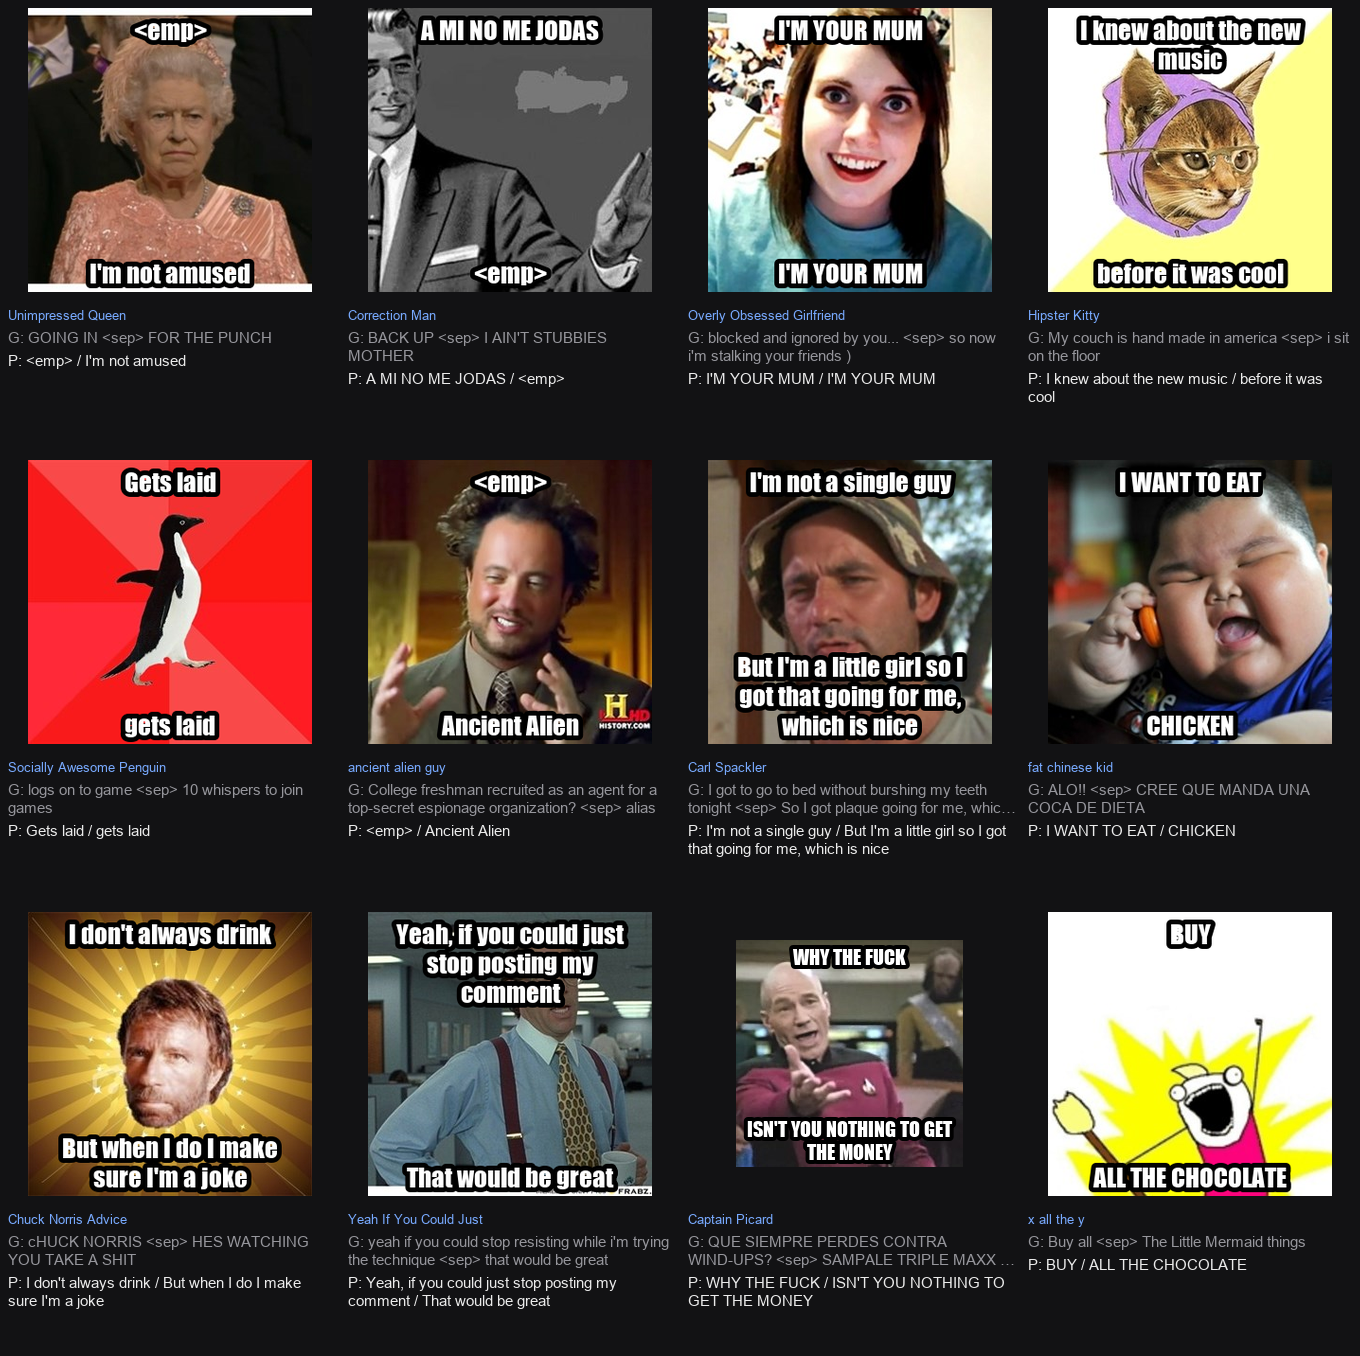
\includegraphics[width=0.95\textwidth]{../showcase/long_clip_transformer_emb768.png}
\caption{Gold vs generated (best run, 3 epochs, embed 768).}
\label{fig:emb}
\end{figure}

\begin{figure}[h]
\centering
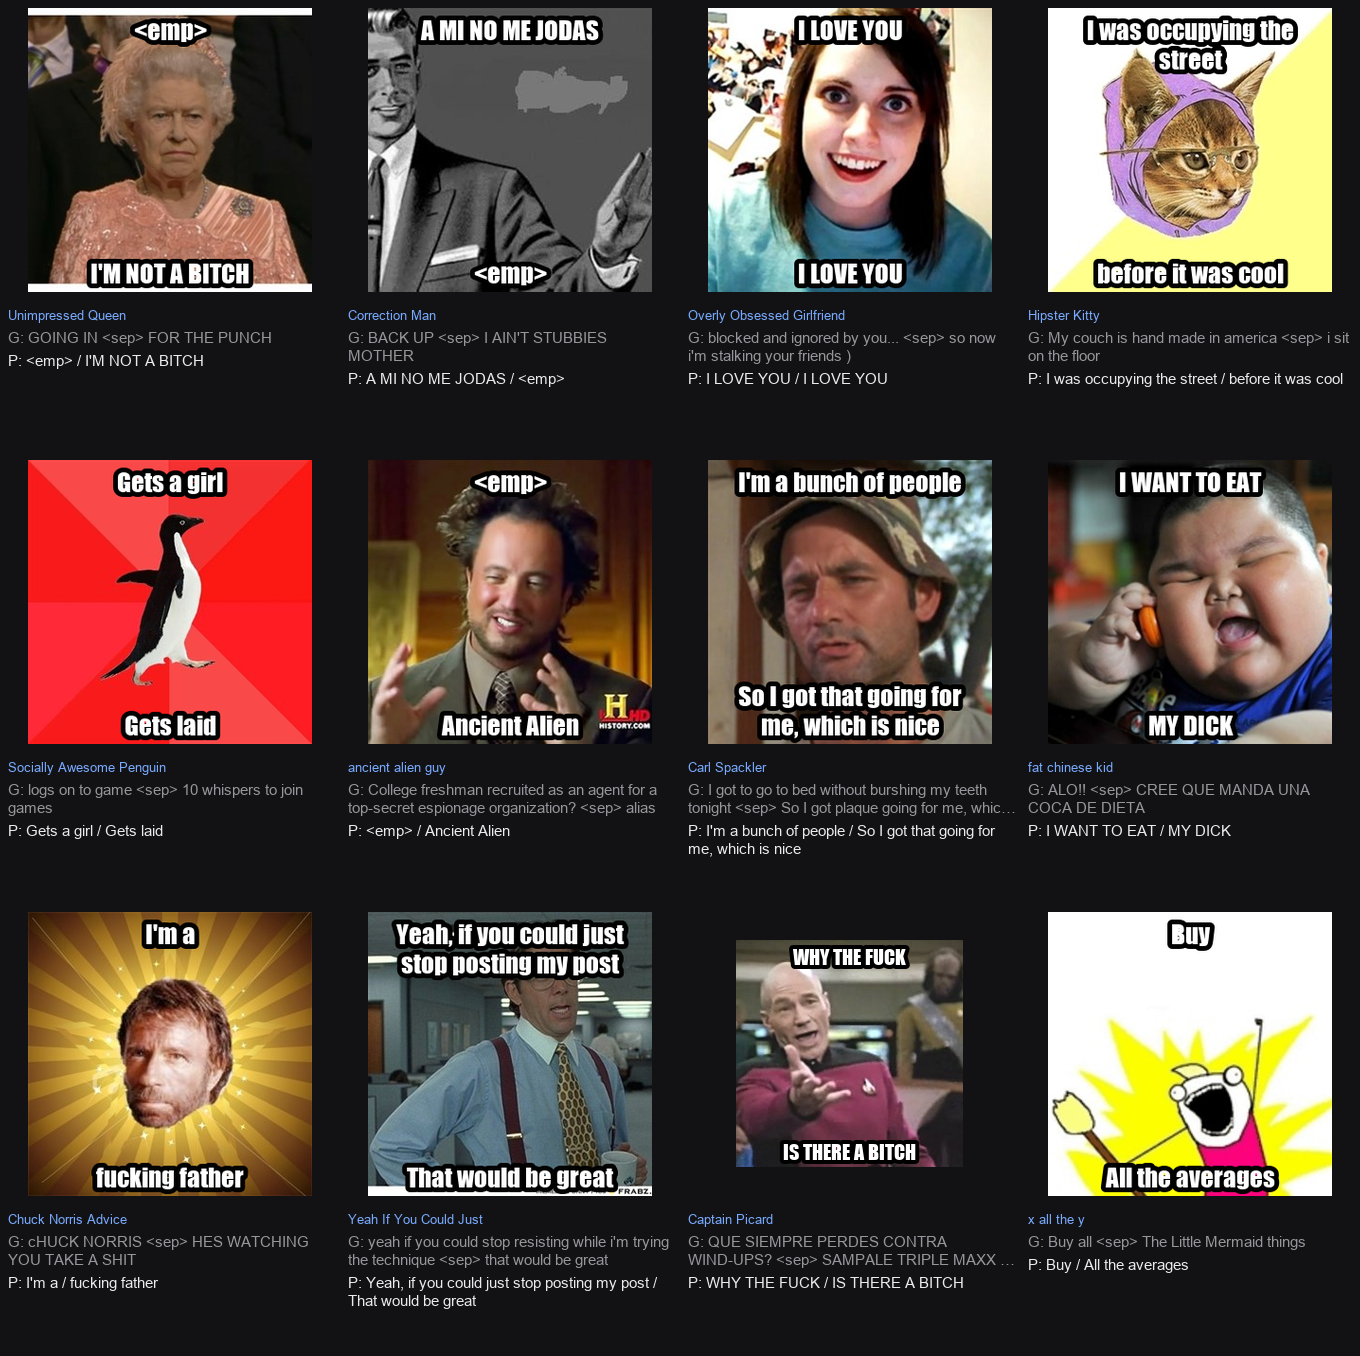
\includegraphics[width=0.95\textwidth]{../showcase/long_resnet50_transformer.png}
\caption{Gold vs generated (ResNet-50 + Transformer, 3 epochs).}
\label{fig:resnet}
\end{figure}

\begin{figure}[h]
\centering
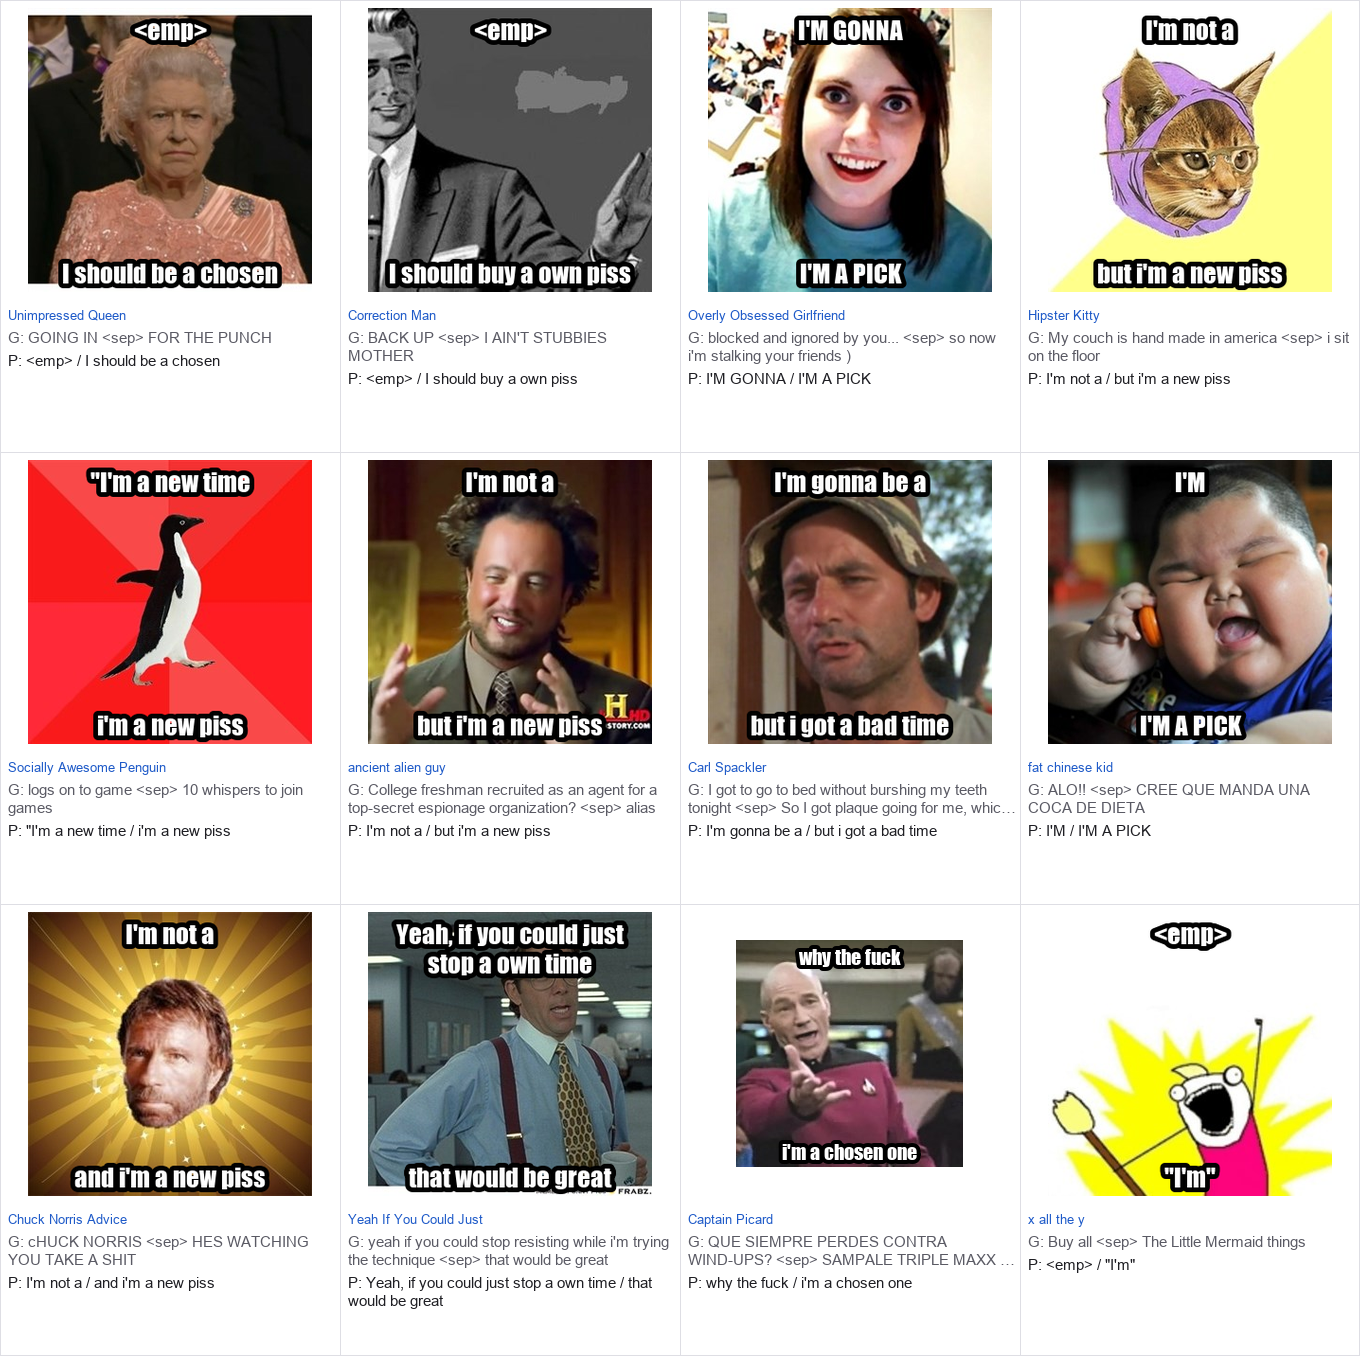
\includegraphics[width=0.95\textwidth]{../showcase/long_clip_lstm.png}
\caption{Gold vs generated (CLIP + LSTM, 3 epochs).}
\label{fig:lstm}
\end{figure}

Interactive: \texttt{./demo.sh} (random template, best checkpoint) or \texttt{caption.py} with a specific image/checkpoint.

\chapter{Discussion}
\label{ch:discussion}

\section{Performance Comparison}
The 2$\times$2 isolates the encoder/decoder: \emph{decoder architecture is the critical choice}. With a Transformer, encoder (ResNet-50 vs CLIP) and embedding size (512 vs 768) have negligible effect at full budget (tight cluster). With an LSTM, CLIP helps substantially at short budget but convergence closes much of the gap at 3 epochs. The screen--confirm split (6k steps to rank by val loss, then confirm at full 1-epoch budget) kept comparisons fair.

\section{Limitations}
\begin{itemize}
\item \textbf{Seen templates only:} caption-level split $\Rightarrow$ scores do not generalize to unseen templates.
\item \textbf{BLEU is harsh for memes:} jokes need not share surface forms; BLEU is meaningful mainly between runs.
\item \textbf{Perplexity not comparable to DeepHumor:} different tokenization (GPT-2 BPE vs dataset-built vocab).
\item \textbf{Task underdetermined:} many valid captions per template; no single ground-truth.
\item \textbf{Exposure bias remains:} teacher forcing vs free-run generation decouple; future work could try scheduled sampling or RL.
\end{itemize}

\chapter{Conclusions and Future Work}
\label{ch:conclusions}

\section{Conclusions}
On \textit{memes900k}, decoder choice dominates: Transformer decoders yield $\sim$14.5 BLEU vs LSTMs at 12--13 after convergence. Behind a Transformer decoder, encoder and embedding size wash out. Perplexity and BLEU decouple (halving perplexity leaves BLEU flat) --- the clearest diagnostic of exposure bias. The main contribution is methodological rigor: test-set BLEU with a shared greedy decoder, the 2$\times$2 isolation, and a two-tier budget, enabling checkable claims.

\section{Future Work}
\begin{itemize}
\item \textbf{Scheduled sampling / REINFORCE:} mitigate exposure bias between training and inference.
\item \textbf{Unseen-template generalization:} evaluate on a held-out template split (harder, truer generalization).
\item \textbf{Better caption metrics:} consider CIDEr/ROUGE or humor-aware proxies, while keeping BLEU for comparability.
\item \textbf{Larger vision encoders / end-to-end fine-tuning:} test whether gains reappear with Transformer decoders.
\item \textbf{Longer budgets and data scaling:} full 750k vs 200k subsample systematically.
\end{itemize}

\begin{appendices}

\chapter{Reproducibility}
\label{app:repro}
\begin{itemize}
\item \textbf{Environment:} Python 3.10, PyTorch, transformers, sacrebleu, numpy, pillow, tqdm (pinned in \texttt{requirements.txt}).
\item \textbf{Offline:} \texttt{HF\_HUB\_OFFLINE=1 TRANSFORMERS\_OFFLINE=1} for training/eval; cached weights/features.
\item \textbf{Data:} \texttt{memes900k/} + \texttt{clip\_features.npz}/\texttt{resnet50\_features.npz}; \texttt{check\_data.py} verifies split.
\item \textbf{Determinism:} fixed seeds; greedy decoding, fixed 5,000-sample test subset; checkpoint stores full args.
\item \textbf{Commands:} train: \texttt{python train.py --encoder <e> --decoder <d> [--epochs N]}; eval: \texttt{python eval.py --checkpoint <ckpt> --split test --out results/<run>.json}; demo: \texttt{./demo.sh}.
\item \textbf{Artifacts:} metrics JSONs in \texttt{results/}, checkpoints in \texttt{checkpoints/}, galleries in \texttt{showcase/}, samples in \texttt{results/samples\_<run>.json}.
\end{itemize}

\end{appendices}

\clearpage\phantomsection\addcontentsline{toc}{chapter}{References}
\bibliographystyle{apacite}
\bibliography{bibliography}

\end{document}
